% =============================================================================
\section{One flight and the chain with one lag}\label{app:single}

\begin{figure*}[t]
\centering
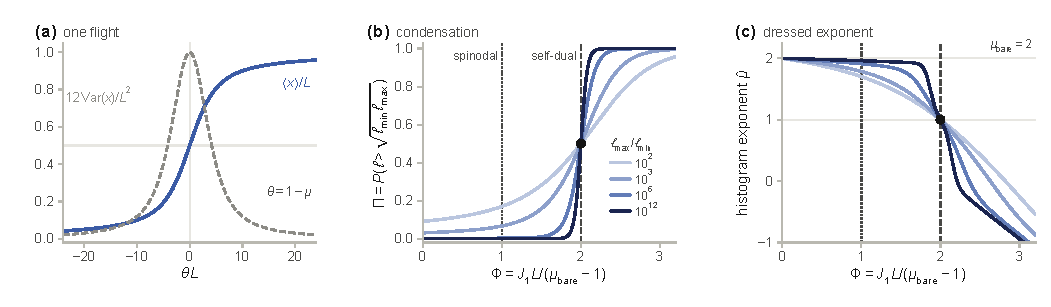
\includegraphics[width=\textwidth]{figs/figA1_theory.pdf}
\caption{The memory chain at depth one. (a)~Response of one flight to its field, Eq.~\eqref{eq:langevin}: mean (solid) and variance (dashed, in units of its maximum $L^2/12$) of $x$. (b)~Order parameter $\Pi$, the fraction of stationary flights longer than $\sqrt{\lmin\lmax}$, versus $\Phi=J_1L/(\mub-1)$ at $\mub=2$, for ranges $\lmax/\lmin$ from $10^2$ to $10^{12}$. The curves cross at the self-dual point $\Phi=2$, $\Pi=1/2$, and sharpen into a step as the range grows; dotted, the spinodal $\Phi=1$. (c)~Exponent returned by an i.i.d.\ truncated-Pareto fit to the same stationary laws: memory lowers it below $\mub$, and every curve crosses $\hat\mu=1$ at $\Phi=2$.}
\label{fig:theory}
\end{figure*}

\paragraph{Single-site law.} For $p(x)\propto e^{\theta x}$ on $[0,L]$, $Z(\theta)=(e^{\theta L}-1)/\theta$ and $\ln Z(\theta)=\theta L/2+\ln[2\sinh(\theta L/2)/\theta]$, so that
\begin{equation}
\frac{d\ln Z}{d\theta}=\frac L2+\frac L2\coth\frac{\theta L}2-\frac1\theta=\Lambda(\theta),\qquad \frac{d^2\ln Z}{d\theta^2}=\Lambda'(\theta),
\end{equation}
which is Eq.~\eqref{eq:langevin} [\figref{fig:theory}(a)]. With $u=2x/L-1$, $p(u)\propto e^{bu}$ on $[-1,1]$ with $b=\theta L/2$, and $\langle u\rangle=\Lang(b)$: this is the law of $\cos\vartheta$ for a classical unit vector with Boltzmann weight $e^{b\cos\vartheta}$, since the area element $\sin\vartheta\,d\vartheta\,d\varphi=-d(\cos\vartheta)\,d\varphi$ is uniform in $\cos\vartheta$. The maximum of $\Lambda'$ is at $\theta=0$, where $\Lang'(0)=1/3$ gives $\Lambda'(0)=L^2/12$. Adding the constraint $\langle x^2\rangle$ gives $p(x)\propto e^{\theta x-\beta x^2}$, a log-normal law truncated to $[\lmin,\lmax]$, which we use as a nested alternative, with integrals computed by Gauss--Legendre quadrature.

\paragraph{Detailed balance.} With $\pi(x)\propto e^{hx}Z(h+Jx)$ and the kernel $p(y|x)=e^{(h+Jx)y}/Z(h+Jx)$,
\begin{equation}
\pi(x)\,p(y|x)\propto e^{hx+(h+Jx)y}=e^{h(x+y)+Jxy},
\end{equation}
which is symmetric in $(x,y)$; $\pi$ is therefore stationary and the chain reversible. Under $x\to L-x$, $y\to L-y$ the exponent becomes $2hL+JL^2-(h+JL)(x+y)+Jxy$, the same weight with $h\to-h-JL$; the self-dual line is $h=-JL/2$.

\paragraph{Path versus causal measure.} The path measure~\eqref{eq:joint} with $K=1$ is a reversible Markov chain whose kernel is the Doob transform of its transfer operator, $p_{\rm path}(y|x)=e^{hy+Jxy}\varphi(y)/[\lambda_0\varphi(x)]$, with $\varphi$ the Perron eigenfunction of the kernel $e^{h(x+y)/2+Jxy}$ on $[0,L]$ and $\lambda_0$ its eigenvalue. The causal kernel is the same expression with $\varphi\equiv1$ and normalization $Z(h+Jx)$. Since $\ln\varphi(y)=J\langle x\rangle_0\,y+O(J^2)$, with $\langle x\rangle_0$ the mean at $J=0$, the two families coincide to first order in $J$ after the shift $h_{\rm causal}=h_{\rm path}+J\langle x\rangle_0$, and they differ at order $J^2$ through an effective log-normal curvature that grows near the thresholds. Fitted to $T=6000$ flights generated by either family, the two return $\hat J=0.095$ and 0.099, with log-likelihoods within 2 nats.

The path measure has the same duality, with self-dual line $h=-JL$ instead of $h=-JL/2$. In the path measure each flight interacts with both its neighbors in time, so a run of flights at the cutoff exerts on a flight a field $h+2JL$, against $h+JL$ in the causal chain, and the self-dual coupling is half as large at the same bare field. The two statements are not in conflict: the bare fields of the two families differ by $J\langle x\rangle_0$, so equal bare fields do not describe the same walk, and only the causal chain is used in this paper. We verified numerically, with the transfer operator on 160 Gauss--Legendre nodes, that on the self-dual line of the path measure $\Pi=1/2$ for every $L$, and that the crossover sharpens with $L$ as for the causal chain.

% -----------------------------------------------------------------------------
\section{Large-range theory of the condensation}\label{app:largeL}

For $\theta L\to+\infty$, $\ln Z(\theta)=\theta L-\ln\theta+o(1)$; for $\theta L\to-\infty$, $\ln Z(\theta)=-\ln|\theta|+o(1)$. With $h=-\alpha$, $J=\beta/L$ and $x=uL$, the field after a flight $x$ is $\theta=-\alpha+\beta u$, and
\begin{equation}
\ln\pi(uL)=-\alpha uL+L\max(\beta u-\alpha,0)+O(\ln L),
\end{equation}
which is Eq.~\eqref{eq:freeenergy}. $F(u)$ is piecewise linear: it increases with slope $\alpha$ for $u<\alpha/\beta$ and, if $\beta>\alpha$, decreases with slope $\alpha-\beta$ beyond. The end $u=1$ is thus a local minimum for $\beta>\alpha$ (spinodal, $J=\Jup$) and the global one for $\beta>2\alpha$ (coexistence, $J=\Jcond$), where $F(1)=2\alpha-\beta$ changes sign. The mass near each minimum is $e^{-LF}$ up to algebraic prefactors, so $\Pi\to\Theta(\beta-2\alpha)$ as $L\to\infty$, a first-order jump. At finite $L$ the exact condition for a secondary maximum of $\pi$ at the cutoff is $J\,\Lambda(h+JL)>\mub-1$, which tends to $J>\Jup$ for wide ranges; below $\Jcond$ its weight is exponentially small, $\pi(L)/\pi(0)\sim e^{(2h+JL)L}$.

Metastability can be seen directly. Starting a chain at $x=L$ in the window $\alpha<\beta<2\alpha$, the first flight shorter than $\sqrt{\lmin\lmax}$ occurs after a mean number of flights that grows exponentially with $L$: at $\beta=1.8\alpha$, from 4 at $\lmax/\lmin=10^2$ to 9 at $10^4$ and 73 at $10^8$ (4000 simulated chains each). In this window a walker that enters a run of long flights stays in it for a time set by the range, the dynamical signature of a metastable phase.

% -----------------------------------------------------------------------------
\section{Estimation}\label{app:estimation}

\paragraph{Likelihood and Newton's method.} Writing $\theta_{i,t}=\bm w\cdot\bm z_{i,t}$, with $\bm w$ collecting fields and couplings and $\bm z_{i,t}$ the corresponding regressors (indicators of the walker or block, lagged flights, covariates), the negative log-likelihood $-l=\sum_{i,t}[\ln Z(\theta_{i,t})-\theta_{i,t}x_{i,t}]$ has gradient $\sum[\Lambda(\theta)-x]\bm z$ and Hessian $\sum\Lambda'(\theta)\,\bm z\bm z^{\mathsf T}$, positive semi-definite. We use Newton's method with a backtracking line search, started from the renewal solution, which converges in a few iterations to a gradient below $10^{-8}$ per flight. The Hessian at the optimum is the observed Fisher information~\eqref{eq:fisher}; the sandwich covariance $\mathsf I^{-1}\mathsf G\,\mathsf I^{-1}$, with $\mathsf G$ the sum of outer products of the per-flight scores, guards against misspecification and is used for the couplings of the fits with one field per walker. All depths $K\le K_{\max}$ are fitted on the same flights, those with at least $K_{\max}$ predecessors, so that they can be compared. The timings quoted in Sec.~\ref{sec:estimation} use a dense Hessian on a single thread.

\paragraph{Centering and the bare exponent.} In the fits the lags are centered, $\theta_t=h+\sum_\tau J_\tau(x_{t-\tau}-c)$, with $c$ the mean of $x$ (of each track, with one field per walker), which decorrelates the field from the couplings. The bare exponent is $\mub=1-h'$, with $h'=h-c\sum_\tau J_\tau$ the field after a run of the shortest flights; its standard error follows from the delta method.

\paragraph{Fields per walker, local fields and covariates.} With one field per walker, $\bm z_{i,t}$ contains the indicator of walker $i$; with local fields, the indicator of the block of $B$ flights to which $t$ belongs (the last block is merged with the previous one if shorter than $B/2$); a known covariate $w_{i,t}$, such as the wall state of a flight, adds a column, $\theta_t\to\theta_t+g\,w_t$. The incidental-parameter bias of the couplings, of order $1/T_i$~\cite{Nickell1981}, is measured on surrogates in which the flights of each walker (or of each block) are permuted, and the $z$-scores of Table~\ref{tab:larvae} are computed against these permutation distributions.

% -----------------------------------------------------------------------------
\section{Model selection and validation}\label{app:selection}

\begin{figure*}[t]
\centering
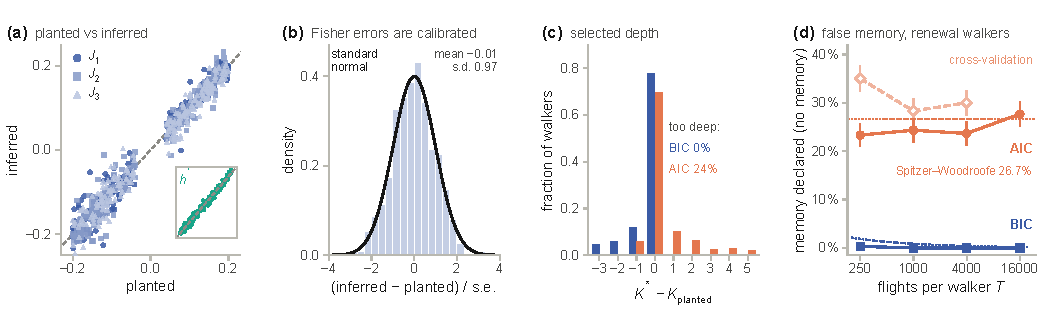
\includegraphics[width=\textwidth]{figs/figA2_validation.pdf}
\caption{Validation on planted walkers. (a)~Planted versus inferred couplings $J_1$, $J_2$, $J_3$ for 200 walkers of $T=3000$ flights, with bare exponents drawn uniformly in $[1.3,2.5]$, couplings of random sign and modulus in $[0.04,0.20]$, and $\lmax/\lmin=10^2$; inset: the field $h'=1-\mub$. (b)~Errors in units of the Fisher standard errors, pooled over all parameters, against the standard normal law. (c)~Selected depth minus planted depth: BIC never overestimates it, and underestimates it only when the last coupling is weaker than about three standard errors; AIC overestimates it in a quarter of the walkers. (d)~Fraction of renewal walkers ($\mub=2$, $\lmax/\lmin=10^3$, 300 replicates per length) declared to have memory by AIC, blocked cross-validation and BIC; dotted lines, the asymptotic values of Eq.~\eqref{eq:woodroofe} for AIC and $P(\chi^2_1>\ln T)$ for BIC.}
\label{fig:validation}
\end{figure*}

\paragraph{AIC and BIC under the null.} For nested models of depths $0,\dots,K_{\max}$, under the null the likelihood-ratio statistics of successive increments are asymptotically independent $\chi^2_1$ variables, so that $\Delta_k=\sum_{j\le k}(\chi^2_{1,j}-2)$ is a random walk with negative drift, and AIC selects the depth at which it is largest. Spitzer's combinatorial lemma gives the probability that the maximum is attained at $k=0$, hence Eq.~\eqref{eq:woodroofe}~\cite{Shibata1976,Woodroofe1982}. Replacing the penalty 2 by $\ln n_{\rm o}$ (BIC) makes the drift diverge, and the false-positive rate decreases as $P(\chi^2_1>\ln n_{\rm o})$ to leading order. Cross-validation with a fixed training fraction estimates the same expected out-of-sample log-likelihood as AIC and is asymptotically equivalent to it~\cite{Stone1977}; it becomes consistent only if the training fraction vanishes~\cite{Shao1993}. Our blocked cross-validation splits each track into five contiguous folds separated by gaps of $K_{\max}$ flights.

\paragraph{Planted walkers.} Walkers generated by the causal chain with random parameters (\figref{fig:validation}) lie along the diagonal of planted versus inferred couplings, and the errors in units of the Fisher standard errors have mean $-0.01$ and standard deviation 0.97. BIC recovers the planted depth in 78\% of the walkers and never selects a deeper one; when it errs, the last coupling is below detection. AIC selects a deeper chain in 24\% of the walkers. On renewal walkers the false-positive rate of AIC stays at the level of Eq.~\eqref{eq:woodroofe} for every length from 250 to 16\,000 flights, that of blocked cross-validation is slightly higher (28--35\%), and that of BIC vanishes as $P(\chi^2_1>\ln T)$. The rates are the same, 21--25\% for AIC and at most 0.5\% for BIC, for exponents $\mu=1.5$--2.5 and for ranges up to five decades.

% -----------------------------------------------------------------------------
\section{What can look like memory}\label{app:pitfalls}

\begin{figure*}[t]
\centering
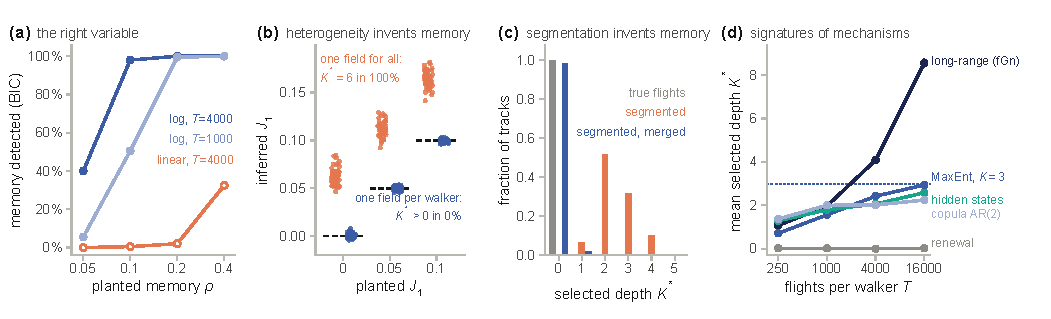
\includegraphics[width=\textwidth]{figs/figA3_pitfalls.pdf}
\caption{How memory is missed or invented, on synthetic walkers. (a)~Power to detect a weak memory with the log statistic $x_tx_{t-1}$ and with the linear statistic $\ell_t\ell_{t-1}$ (BIC; 200 replicates per point). (b)~Inferred lag-1 coupling for 40 walkers with individual exponents $\mu_i\sim U(1.2,2.2)$ and $T=1000$ flights each, with a common field (coral) or one field per walker (indigo); dashed, planted values. (c)~Selected depth for a renewal L\'evy walk sampled at fixed times with localization noise: true flights, flights segmented from the track, and segmented flights after merging nearly collinear pieces. (d)~Mean selected depth ($\pm$ s.e.) versus the number of flights for five mechanisms with truncated-Pareto marginals: renewal, a MaxEnt chain of depth 3 (dotted: its true depth), a Gaussian-copula AR(2) process, a walker switching between two hidden states, and long-range memory (Gaussian copula of fractional Gaussian noise with Hurst exponent 0.75).}
\label{fig:pitfalls}
\end{figure*}

\paragraph{The variable.} The statistic $\ell_t\ell_{t-1}$, the natural guess in linear space, is dominated by a handful of extreme flights. For a weak memory, a Gaussian-copula autoregression with truncated-Pareto marginals and correlation $\rho=0.1$ ($T=4000$), the log statistic $x_tx_{t-1}$ detects it in 98\% of the walkers and the linear one in none [\figref{fig:pitfalls}(a)].

\paragraph{Heterogeneity.} With 40 memoryless walkers whose exponents are spread over $[1.2,2.2]$, a model with a common field selects the maximal depth in every replicate and returns $J_1\simeq0.11$ for a planted $0.05$. One field per walker removes both the false positives and the bias [\figref{fig:pitfalls}(b)].

\paragraph{Corridor segmentation.} Positions are sampled at fixed times with noise, and flights must be cut out of the track. A flight is the longest stretch of track that stays within a corridor of half-width $\varepsilon$ around the segment joining its end points~\cite{Rhee2011,Humphries2013}; the track is scanned from its start, each flight being extended until a point leaves the corridor, and its length is the distance between its end points.

\paragraph{Merging.} Localization noise displaces single points out of the corridor and splits a long flight into two long pieces, a positive correlation between consecutive lengths that the analysis reads as memory: a renewal L\'evy walk segmented in this way shows $K^*=2$--3 [\figref{fig:pitfalls}(c)], and the lag-1 autocorrelation of $\ln\ell$ rises from 0.02 to 0.21. We merge consecutive pieces whose headings differ by less than $\theta_c=20^\circ$, which restores $K^*=0$ while leaving genuine memory detectable. Applied to true flights with independent turning angles, merging deletes boundaries independently of the lengths, an i.i.d.\ thinning of the renewal process, which therefore remains renewal; applied to noise-split pieces, it restores the original flights. The test of \figref{fig:pitfalls}(c) uses renewal L\'evy walks of 3000 flights with $\mu=2$ over three decades, uniformly random directions and unit speed, sampled at $\Delta t=0.25$ with Gaussian localization noise of standard deviation 0.02, and segmented with $\varepsilon=0.1$ and $\lmin=1$.

\paragraph{Pipeline null.} On real data the track is cut at its flight boundaries; the pieces, each with its own sub-sampled points, are reshuffled, rotated, and reconnected with turning angles drawn from the empirical distribution; the whole pipeline (segmentation, merging, fit) is then run again on the rebuilt track. Any memory found there is produced by the pipeline.

\paragraph{Signatures of mechanisms.} Mechanisms of dependence differ in how the selected depth grows with the length of the data [\figref{fig:pitfalls}(d)]. $K^*$ stays at zero for a renewal walk and saturates at the true order for a finite memory. It grows slowly for a walker that switches between hidden states, whose dependence decays geometrically and becomes resolvable lag after lag, and without bound for long-range memory.

% -----------------------------------------------------------------------------
\section{Data sets and controls on single walkers}\label{app:data}

\begin{table}[b]
\caption{Data sets.}
\label{tab:datasets}
\begin{ruledtabular}
\begin{tabular}{>{\raggedright\arraybackslash}p{2.0cm}>{\raggedright\arraybackslash}p{6.2cm}}
system & content and source\\
\colrule
\emph{Drosophila} larvae & 304 tracks at 2\,Hz, up to 1\,h, 10 genotype--temperature conditions, $240\times240$\,mm agar arenas~\cite{Sims2019}; Dryad doi:10.5061/dryad.7m0cfxpq0, mirror Zenodo 4996872 (CC0)\\
termite workers & 75 focal \emph{C.~cumulans} workers, 2\,Hz for 6\,h, Petri dishes of $\approx49$\,mm~\cite{Castiblanco2019}; Zenodo 3628061 (CC-BY 4.0)\\
T cells & 1106 tracks of zebrafish and mouse T cells and \emph{Dictyostelium}~\cite{Jerison2020}; GitHub erjerison/TCellMigration (MIT)\\
baboons & 26 GPS-collared members of a troop of olive baboons (\emph{Papio anubis}), 1\,Hz from 06:00 to 18:00 on 14 days~\cite{StrandburgPeshkin2015}; Movebank Data Repository doi:\allowbreak 10.5441/\allowbreak 001/1.kn0816jn (CC0)~\cite{Crofoot2015data}\\
pigeons & three flocks of homing pigeons (6, 10 and 8 tracked birds), 41 releases, GPS at 1\,Hz (5\,Hz for some birds)~\cite{MehlhausenFranks2025}; Dryad doi:\allowbreak 10.5061/\allowbreak dryad.4tmpg4fp6 (CC0)~\cite{MehlhausenFranks2025data}\\
\end{tabular}
\end{ruledtabular}
\end{table}

\begin{table*}[t]
\caption{Memory between consecutive flights of \emph{Drosophila} larvae. BL drives expression in the brain lobes and part of the subesophageal ganglion, BLsens also in all sensory neurons, MB247 in the mushroom bodies; ``shi'' is the temperature-sensitive \emph{shibire}$^{ts}$, which silences the targeted neurons at 33\,$^\circ$C, and \emph{rpr,hid} the pro-apoptotic genes that kill them; X/+ and shi/+ carry a single transgene. $K^*$: depth selected by BIC with one field per larva. $J_1$: lag-1 coupling of the fit with $K=1$ ($\pm$ s.e.). $z_{\rm sh}$: $J_1$ against 30 within-larva permutations of the flights. $z_{25}$: the same with fields re-estimated every 25 flights, against permutations within blocks (truncated power law / truncated log-normal single-flight law). $\Phi=J_1L/(\mub-1)$: median over larvae. The permutation null selects $K^*>0$ in 1 of 300 surrogates, the pipeline null in none of 50.}
\label{tab:larvae}
\begin{ruledtabular}
\begin{tabular}{llrrcr@{\,$\pm$\,}lrrr}
condition & manipulation & larvae & flights & $K^*$ & \multicolumn{2}{c}{$J_1$} & $z_{\rm sh}$ & $z_{25}$ & $\Phi$\\
\colrule
BL/+, 22\,$^\circ$C & control & 24 & 1976 & 0 & $-0.004$ & 0.019 & 0.2 & 0.3 / 0.1 & 0.07\\
shi/+, 22\,$^\circ$C & control & 19 & 1366 & 0 & 0.088 & 0.030 & 3.2 & 3.3 / 3.5 & 0.56\\
\emph{rpr,hid} control & control & 59 & 4240 & 1 & 0.074 & 0.012 & 12.3 & 6.6 / 8.2 & 0.77\\
BL/+, 33\,$^\circ$C & control & 26 & 2337 & 1 & 0.071 & 0.016 & 5.3 & 3.6 / 4.8 & 0.69\\
shi/+, 33\,$^\circ$C & control & 29 & 2605 & 1 & 0.127 & 0.013 & 11.2 & 10.4 / 7.4 & 1.02\\
MB247/+ & control & 21 & 1630 & 2 & 0.139 & 0.021 & 7.7 & 6.4 / 6.5 & 0.86\\
MB247$>$shi & mushroom bodies silenced & 22 & 2103 & 3 & 0.168 & 0.021 & 9.7 & 8.3 / 6.7 & 1.04\\
BL$>$shi & brain lobes silenced & 17 & 2366 & 4 & 0.058 & 0.025 & 2.8 & $-2.1$ / $-2.3$ & 0.35\\
BLsens$>$shi & brain lobes and sensory neurons silenced & 6 & 349 & 0 & $-0.063$ & 0.106 & $-0.2$ & $-2.2$ / $-1.9$ & $-0.32$\\
BLsens$>$\emph{rpr,hid} & brain lobes and sensory neurons ablated & 18 & 1976 & 2 & 0.307 & 0.045 & 8.2 & 5.0 / 4.0 & 0.72\\
\end{tabular}
\end{ruledtabular}
\end{table*}

\begin{figure*}[t]
\centering
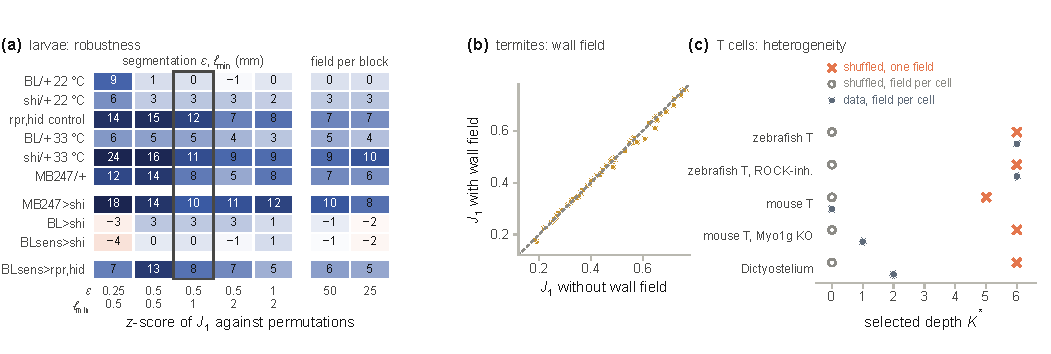
\includegraphics[width=\textwidth]{figs/figA4_controls.pdf}
\caption{Controls on real walkers. (a)~\emph{Drosophila} larvae: $z$-score of $J_1$ against permutation nulls for five segmentation settings (corridor half-width $\varepsilon$ and $\lmin$, in mm; boxed, the setting of Table~\ref{tab:larvae}), and with fields re-estimated every 50 or 25 flights, against permutations within blocks. (b)~Termites: lag-1 coupling of a $K=1$ fit with and without a wall field (band of 6\,mm), one point per termite. (c)~T cells and \emph{Dictyostelium}~\cite{Jerison2020}: depth selected after shuffling the steps within each cell, with a common field (crosses) or one field per cell (open circles), and on the real data with one field per cell (filled).}
\label{fig:controls}
\end{figure*}

\paragraph{Preprocessing.} Table~\ref{tab:datasets} lists the data. For the larvae, flights below $\lmin=1$\,mm (5--13\% of all flights, 28\% for the two lines with silenced or ablated sensory neurons) are set to $\lmin$, and $\lmax$ is the longest flight of the condition. For the termites, $\lmax$ is the longest flight of each track (26--45\,mm), and the wall state of a flight is the fraction of its points within 3, 6 or 9\,mm of the wall, the arena being estimated from the track as the circle that contains 99.5\% of its points. For the T cells the variable is the displacement per frame, with $\lmin$ at the 5th percentile. For the collective analyses, $\lmin$ is at the localization floor (5th percentile) and steps above the 99.95th percentile are treated as tracking glitches. Baboon positions are taken every 10\,s (every 30\,s for the robustness check) and pigeon positions every second, keeping the first fix of each second for the birds logged at 5\,Hz. A heading is defined for steps of at least 1\,m (baboons, about four times the GPS error) or 3\,m (pigeons); a unit that moves less contributes a zero vector to its own lags and to its neighbors' regressors. Each day (baboons) or release (pigeons) is a co-recorded group, with its own unit and time fields.

\paragraph{Larvae.} Table~\ref{tab:larvae} details the ten conditions. The memory does not depend on the segmentation, with $\varepsilon\in\{0.25,0.5,1\}$\,mm and $\lmin\in\{0.5,1,2\}$\,mm, and in six of the seven conditions with memory it survives fields re-estimated every 50 or 25 flights [\figref{fig:controls}(a)]; in BL$>$shi it does not. Over the full range $[\lmin,\lmax]$ a truncated log-normal law, the MaxEnt law with $\langle x^2\rangle$ also fixed, describes the histogram better than a truncated power law in eight conditions out of ten ($\Delta$BIC$\,=286$--1625); the power law is competitive only for the larvae with silenced or ablated sensory neurons. This does not contradict tail fits above a data-chosen $x_{\min}$~\cite{Clauset2009}, but ``L\'evy'' here refers to two decades at most. The memory is the same with either single-flight law (Table~\ref{tab:larvae}, $z_{25}$).

\paragraph{Termites and the wall.} With the wall state of each flight as a covariate, the lag-1 coupling is unchanged in every termite [\figref{fig:controls}(b)]. The wall field improves BIC by a few units for the typical termite (median $-3.5$ at 6\,mm) and by much more for a few, without affecting their memory.

\paragraph{T cells.} With a common field, shuffled T cells select $K^*=5$--6 in 49 of 50 surrogates, the maximal depth in 43; with one field per cell, $K^*=0$ in every surrogate [\figref{fig:controls}(c)]. The steps are log-normal rather than power-law distributed, by $10^2$--$10^4$ BIC units.

% -----------------------------------------------------------------------------
\section{The collective model}\label{app:collective}

\begin{figure*}[t]
\centering
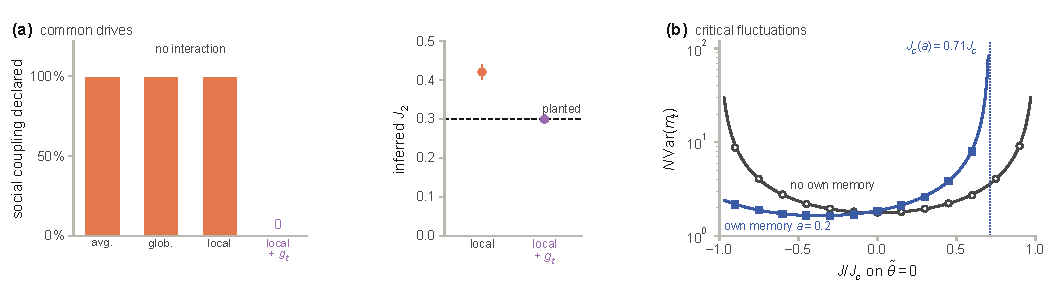
\includegraphics[width=\textwidth]{figs/figA5_collective.pdf}
\caption{Synthetic collectives. (a)~A drive common to all units, without interaction (40 replicates): fraction of data sets in which a social coupling is declared by the group-average analysis, by a global coupling, by a local coupling, and by a local coupling with time fields; right, a planted local coupling $J_2=0.3$ under the same drive, inferred without and with time fields (mean $\pm$ s.d.). (b)~Fluctuations of the collective log-speed versus $J$ on the line $\tilde\theta=0$, without (open circles) and with own memory $a=0.2$ (squares); lines, the theory of Sec.~\ref{sec:meanfield}; dotted, the shifted threshold $J_c(a)=0.71J_c$. $L=\ln100$.}
\label{fig:collective}
\end{figure*}

\begin{table*}[t]
\caption{Synthetic collectives: the analysis of the group average of Ref.~\cite{Agliari2024} (depth $\tau_M^*$ selected by AIC, delay given by $\arg\max_\tau|J_\tau|$) against the self\,+\,social model~\eqref{eq:selfsocial} (depths by BIC). ``Declared'': a nonzero social coupling is selected. Speed-Vicsek model, $L=\ln100$, 1500 frames, $N=50$ unless stated; replicates in parentheses.}
\label{tab:collective}
\begin{ruledtabular}
\begin{tabular}{>{\raggedright\arraybackslash}p{5.0cm}>{\raggedright\arraybackslash}p{5.6cm}>{\raggedright\arraybackslash}p{5.6cm}}
experiment & group average & self\,+\,social\\
\colrule
own memory $a=(0.25,0.10)$, local $J_3=0.35$ (40) & delay 3 in 22/40, 1 in 13/40; spurious $J_1=0.28$, $J_2=0.12$ & $(K_s^*,K_c^*)=(2,3)$ in 38/40; $\hat a=(0.245,0.095)$, $\hat J_3=0.348\pm0.024$\\
own memory of depth 3, no interaction ($N=10$, 30, 100; 40 each) & declared in 100\% (exact likelihood: 97--100\%) & declared in 1/120; $K_s^*=3$ in 116/120\\
common drive, no interaction (40) & declared in 100\% & global 100\%, local 100\%, local with time fields 0\%\\
common drive, local $J_2=0.3$ (40) & declared in 100\% & local: $\hat J_2=0.42$; local with time fields: $\hat J_2=0.300\pm0.012$\\
group-average model true, $J_1=0.25$, $J_4=0.35$ ($N=5$--100; 60 each) & $\hat J_4=0.43\pm0.06$ at $N=5$, $0.35\pm0.04$ at $N=100$ & exact likelihood: $\hat J_4=0.34\pm0.03$ at $N=5$, $0.35\pm0.04$ at $N=100$\\
own memory, local delay $\Delta=1,2,4,6$ (30 each) & delay recovered in 100, 73, 40, 17\% & delay recovered in 100\% for every $\Delta$\\
directions, persistent turning, no interaction (30) & declared in 30/30 (delay 1) & declared in 0/30\\
directions, persistence and local $J_3$ (30) & delay 3 in 0/30 (always 1) & declared in 30/30, delay 3 in 30/30\\
\end{tabular}
\end{ruledtabular}
\end{table*}

\paragraph{Estimation.} The self\,+\,social model~\eqref{eq:selfsocial} is fitted by Newton's method with a sparse Hessian (unit and time fields) and a dense block for the shared couplings. The block of the time fields is diagonal, because each row belongs to one frame, so each Newton step eliminates it exactly (a Schur complement) and solves the remaining dense system for unit fields and couplings, a few hundred parameters; with $6\times10^4$ time fields (baboons at 10\,s) a fit takes seconds, with the same optimum and standard errors as a sparse factorization. Unit and time fields have one flat direction per co-recorded group, $h_i\to h_i+\Delta$, $g_t\to g_t-\Delta$, fixed by a vanishing ridge on the $g_t$; the flat directions are common to all models compared, so BIC differences are unaffected. Self and social depths are selected jointly by BIC on common rows. For directions, $p(\bm n_i^t|\text{past})\propto e^{\bm\theta_i^t\cdot\bm n_i^t}$ is a von Mises law~\cite{MardiaJupp2000} for the unit vector $\bm n_i^t$ of the step, with $\bm\theta_i^t=\mathbf h_i+\mathbf g_t+\sum_\tau a_\tau\bm n_i^{t-\tau}+\sum_\tau J_\tau\bm s_i^{t-\tau}$, the planar spin of Ref.~\cite{Agliari2024}, where $\bm s_i^{t-\tau}$ is the mean unit vector of the neighbors; its negative log-likelihood $\sum[\ln I_0(|\bm\theta|)-\bm\theta\cdot\bm n]$ is convex, and the time-field block is two-by-two block diagonal.

\paragraph{Exactness of the mean-field measure.} The measure $P_A$ of Ref.~\cite{Agliari2024} factorizes over units and frames with one-body weights $e^{x_i^t\theta_t}/Z(\theta_t)$, the first $\tau_M$ frames being fixed by delta functions; evaluated at the data it is $\prod_{t,i}p(x_i^t|\text{past})$ with $\theta_t=H+\sum_\tau J_\tau m^E_{t-\tau}$. Concavity follows as for Eq.~\eqref{eq:loglik}. The stationarity conditions $\sum_{t,i}[x_i^t-\Lambda(\theta_t)]=0$ and $\sum_{t,i}[x_i^t-\Lambda(\theta_t)]m_{t-\tau}=0$ characterize the exact estimator, whereas the original implementation~\cite{Agliari2024} imposes $\Lambda(\theta_t)\simeq m_t$ frame by frame and solves it by least squares after the inversion $G_t=\Lambda^{-1}(m_t)$, a convenient moment approximation.

\paragraph{Aggregation.} Let units be conditionally independent given their own pasts and jointly stationary. For a model of the group average alone, the expected score for $J_\tau$ at $J=0$ is $\E[\sum_i(x_i^t-\bar m)m_{t-\tau}]=N^{-1}\sum_{i,j}\mathrm{Cov}(x_i^t,x_j^{t-\tau})=\bar C(\tau)$ per frame, of order one: $J=0$ is not a solution whenever there is own memory. Linearizing $G_t\simeq\bar\theta+(m_t-\bar m)/\Lambda'(\bar\theta)$, the regression of $G_t$ on lags of $m$ is $1/\Lambda'$ times the autoregression of $m$ on its own lags; since $\mathrm{Cov}(m_t,m_{t-\tau})=N^{-1}\bar C(\tau)$, the factors $N^{-1}$ cancel in the Yule--Walker equations, which gives Eq.~\eqref{eq:aggregation}. For the self\,+\,social model with leave-one-out regressors, the tower property gives $\E[(x_i^t-\E[x_i^t|x_i^{<t}])\,m^{(-i)}_{t-\tau}]=0$, because $m^{(-i)}$ is independent of unit $i$: the social score vanishes at the truth.

\paragraph{Common drives.} A shared stationary field $u_t$ with autocovariance $C_u$ induces $\mathrm{Cov}(x_i^t,x_j^{t-\tau})\simeq\Lambda'^2C_u(\tau)$ between non-interacting units, to linear order. With unit and time fields, the identity $m^{(-i)}_{t-\tau}=\frac{n}{n-1}m_{t-\tau}-\frac1{n-1}x_i^{t-\tau}$ ($n$ units in the frame) shows that the global regressor is a function of the frame, absorbed by $g_t$, plus a multiple of the own lag. For $\tau\le K_s$ a global coupling is not identifiable (exactly so when $n$ is constant); for $\tau>K_s$ it estimates $-(n-1)$ times the omitted own memory at that lag. A local regressor is not in the span of the time fields and own lags unless all neighborhood means coincide. On synthetic data [\figref{fig:collective}(a)], every reading except local coupling with time fields declares a coupling under a common drive alone, and only that reading recovers a planted local coupling without bias.

\paragraph{Mean-field theory.} By the law of large numbers, $m_t\to\Lambda(H+\sum_\tau J_\tau m_{t-\tau})$. Linearizing around a fixed point gives the characteristic equation $1=\Lambda'(\theta^*)\sum_\tau J_\tau z^{-\tau}$. For non-negative couplings, $f(z)=\Lambda'\sum_\tau J_\tau z^{-\tau}$ is decreasing on $z>0$ and $|f(z)|\le f(|z|)$, so a root with $|z|\ge1$ exists if and only if $f(1)=\Lambda'J_{\rm tot}\ge1$; when the delays have no common divisor the critical root is $z=1$ alone (a fold). Since $\Lambda'\le L^2/12$, with equality at $\theta=0$, bistability requires $J_{\rm tot}>12/L^2$, the cusp being at $\tilde\theta=0$, $m=L/2$. For a single delay $d$ the map decouples into $d$ sub-chains $y^{(r)}_n=m_{nd+r}$ obeying $y_{n+1}=\Lambda(H+Jy_n)$; for $J<0$ each undergoes a flip at $\Lambda'|J|=1$, and a lag-1 term $a_1>0$ in the characteristic equation $z^d=\Lambda'J+\Lambda'a_1z^{d-1}$ favors the in-phase mode, of period $2d$. For finite $N$ and one lag, $\delta m_t=\Lambda'J\delta m_{t-1}+\eta_t$ with $\mathrm{Var}\,\eta=\Lambda'/N$ gives $N\,\mathrm{Var}(m)=\Lambda'/[1-(\Lambda'J)^2]$ [\figref{fig:collective}(b)].

\paragraph{Own memory in mean field.} With lag-1 self coupling $a\ge0$, propagation of chaos makes each unit, at a stationary state $m^*$, an independent chain with field $h_{\rm eff}=H+J_{\rm tot}m^*$ and stationary law $\pi(x)\propto e^{h_{\rm eff}x}Z(h_{\rm eff}+ax)$, Eq.~\eqref{eq:stationary}. The self-consistency is $m^*=\Psi(H+J_{\rm tot}m^*)$, with $\Psi(h)=\E_\pi[x]$, and the symmetry line is $H+(J_{\rm tot}+a)L/2=0$. A field perturbation propagates as $\delta m_t=\sum_{s\ge0}R(s)\,\delta h_{t-s}$, with $R(s)=\mathrm{Cov}(x_s,\epsilon_0)$ the response of one unit, $\epsilon_0=x_0-\E[x_0|\text{past}]$ being the innovation; for $a\ge0$, $R(s)\ge0$, the argument above applies to $1=\hat R(z)\sum_\tau J_\tau z^{-\tau}$, and stability is lost at $J_{\rm tot}\chi=1$ with $\chi=\sum_sR(s)=\partial\Psi/\partial h$. To leading order in $1/N$, $N\,\mathrm{Var}(m)=\int\frac{d\omega}{2\pi}S_x(\omega)|1-\hat J(\omega)\hat R(\omega)|^{-2}$, with $S_x$ the spectrum of one unit. We compute $R$, $S_x$ and $\chi$ from the transition matrix of the chain on 400 Gauss--Legendre nodes.

\paragraph{Synthetic collectives.} The speed-Vicsek model places $N$ units in a periodic box; headings follow Vicsek alignment~\cite{Vicsek1995}, and log-speeds are drawn from Eq.~\eqref{eq:selfsocial} with planted own memory, local (three nearest neighbors) or global couplings and, when stated, a common Ornstein--Uhlenbeck drive; steps are then recomputed from the positions, as in an experiment. Individual fields are drawn from $U(-1.3,-0.5)$. Table~\ref{tab:collective} collects the experiments. Directions behave like speeds: for units with persistent turning and no interaction, the group-average analysis of directions declares delayed interactions in every replicate, the self\,+\,social von Mises model in none. With AIC instead of BIC, the self\,+\,social model itself declares spurious couplings in 27\% of interaction-free data sets, the value of Eq.~\eqref{eq:woodroofe} again.

\paragraph{Time-shift null.} In a time-shift surrogate every unit's track is shifted by an independent random circular offset, which keeps its own memory, heterogeneity and marginal law and destroys every synchrony between units, interactions and common drives alike; a permutation of frames destroys own memory as well, and therefore tests memory and synchrony together.

\paragraph{Neighbors in real groups.} The local regressor of unit $i$ at delay $\tau$ is the mean of the variable over the units of distance ranks $r_0+1,\dots,r_1$ from $i$ at the emission frame $t-\tau$: the three nearest for baboons, and the nearest one for pigeons, whose flocks have three to eight birds in a frame, so that a larger neighborhood would be the whole flock and, as shown above, not identifiable with time fields. The decay with distance is measured by single-neighbor regressors of ranks 1, 2, 3, 6 and 12 (baboons) or 1, 2 and 3 (pigeons), fitted jointly with three delays each; the asymmetry, by splitting the six (baboons) or three (pigeons) nearest neighbors into those ahead of and those behind $i$ along the group heading, the direction of the mean step at $t-\tau$. Anchoring the neighborhood at the current position of $i$ instead (the units that at $t-\tau$ were nearest to where $i$ is now) also picks up fields fixed in space, such as trails, which time fields cannot absorb. In the time-shift null the positions are shifted with the steps, so the neighbors of a shifted unit are whoever passed near the same place at another time: the null removes synchrony but keeps fields fixed in space, and its coupling to the nearest neighbor need not vanish.
